%%%%%%%%%%%%%%%%%%%%%%%%%%%%%%%%%%%%%%%%%%%%%%%%%%%%%%%%%%%%%%%%%%%%%%%%%%%%%%%
%% SOCIOL 723 -- Social Statistics II
% Week 7 -- Instrumental Variables
%% Wenhao Jiang, Duke University, Fall 2026
%%%%%%%%%%%%%%%%%%%%%%%%%%%%%%%%%%%%%%%%%%%%%%%%%%%%%%%%%%%%%%%%%%%%%%%%%%%%%%%

\documentclass[aspectratio=169,11pt,xcolor=dvipsnames]{beamer}
\mode<presentation>

%% ---- fonts: Latin Modern Roman (the LaTeX default), serif throughout -------
\usepackage[T1]{fontenc}
\usepackage{lmodern}
\usefonttheme{serif}
\renewcommand{\familydefault}{\rmdefault}

%% ---- packages --------------------------------------------------------------
\usepackage{amsmath,amsfonts,amssymb,bm}
\usepackage{graphicx}
\usepackage{booktabs}
\usepackage{tikz}
\usetikzlibrary{arrows.meta,positioning,calc}
\usepackage[english]{babel}

\newcommand{\srcp}[1]{{\scriptsize\color{gray}(#1)}}
\newcommand{\srct}[1]{#1}

\DeclareMathOperator*{\argmin}{arg\,min}
\DeclareMathOperator*{\argmax}{arg\,max}
\DeclareMathOperator{\Cov}{Cov}
\DeclareMathOperator{\Var}{Var}
\DeclareMathOperator{\trace}{tr}
\DeclareMathOperator{\rank}{rank}
\DeclareMathOperator{\plim}{plim}
\newcommand{\indep}{\perp\!\!\!\perp}

%% ---- notation conventions (course-wide) ------------------------------------
\newcommand{\E}{E}
\newcommand{\En}{\mathbb{E}_n}
\newcommand{\R}{\mathbb{R}}
\newcommand{\X}{\bm{X}}
\newcommand{\Y}{\bm{y}}
\newcommand{\Ix}{\bm{I}}
\newcommand{\zero}{\bm{0}}
\newcommand{\bhat}{\hat{\bm{\beta}}}
\newcommand{\dto}{\overset{d}{\longrightarrow}}
\newcommand{\pto}{\overset{p}{\longrightarrow}}
\usetikzlibrary{shapes,decorations.pathmorphing}
\newcommand{\lik}{\mathcal{L}}
\newcommand{\loglik}{\ell}
\newcommand{\Info}{\mathcal{I}}
\newcommand{\SE}{\widehat{\text{SE}}}

%% ---- theme -----------------------------------------------------------------
\usetheme{default}
\useoutertheme[subsection=false]{miniframes}
\setbeamertemplate{mini frames}{}

\definecolor{dukeblue}{RGB}{1,33,105}
\definecolor{accent}{RGB}{200,78,0}
\definecolor{softgray}{RGB}{242,242,245}

\setbeamercolor{structure}{fg=dukeblue}
\setbeamercolor{frametitle}{fg=dukeblue,bg=white}
\setbeamercolor{section in head/foot}{fg=white,bg=dukeblue}
\setbeamercolor{alerted text}{fg=accent}
\setbeamercolor{block title}{fg=white,bg=dukeblue}
\setbeamercolor{block body}{fg=black,bg=softgray}
\setbeamercolor{block title alerted}{fg=white,bg=accent}
\setbeamercolor{block body alerted}{fg=black,bg=softgray}

\setbeamertemplate{footline}[page number]
\setbeamertemplate{navigation symbols}{}
\setbeamertemplate{itemize items}[circle]
\setbeamertemplate{blocks}[rounded][shadow=false]
\setbeamerfont{frametitle}{series=\bfseries}
\setbeamerfont{footnote}{size=\scriptsize}
\setbeamerfont{caption}{size=\footnotesize}
\setbeamertemplate{subsection in head/foot}{}
\setbeamertemplate{subsection in head/foot shaded}{}
\setbeamertemplate{caption}[numbered]

\newcommand{\adv}{\,\raisebox{0.6pt}{\textcolor{accent}{$\bigstar$}}}

\setbeamertemplate{section page}{%
  \begin{centering}\vfill
  {\usebeamercolor[fg]{structure}\Large\bfseries\insertsectionhead\par}
  \vskip4pt{\color{dukeblue}\rule{0.35\linewidth}{1pt}\par}
  \vfill\end{centering}}
\setbeamertemplate{subsection page}{%
  \begin{centering}\vfill
  {\usebeamercolor[fg]{structure}\large\bfseries\insertsubsectionhead\par}
  \vfill\end{centering}}

\AtBeginDocument{%
  \setlength{\abovedisplayskip}{5pt}%
  \setlength{\belowdisplayskip}{5pt}%
  \setlength{\abovedisplayshortskip}{2pt}%
  \setlength{\belowdisplayshortskip}{3pt}%
}
\setbeamertemplate{frametitle}{%
  \vskip4pt\usebeamerfont{frametitle}\usebeamercolor[fg]{frametitle}%
  \insertframetitle\par\vskip2pt}
\setbeamersize{text margin left=0.75cm, text margin right=0.75cm}

%% ---- title -----------------------------------------------------------------
\title[SOCIOL 723]{SOCIOL 723: Social Statistics II\\[2pt]}
\subtitle{\large Week 7 --- Instrumental Variables\\[-8pt]}
\author[Jiang]{\large Wenhao Jiang\vspace{-1.5em}}
\institute[Duke]{}
\titlegraphic{
\includegraphics[height=1.3cm]{../Misc/duke_logo.png}}
\date{\large Department of Sociology, Fall 2026}



\begin{document}

\begin{frame}[plain]
  \titlepage
\end{frame}

\begin{frame}{Today}
  \tableofcontents
\end{frame}

\begin{frame}{A Change of Strategy}
Week 6 assumed we had measured every confounder and worked on \emph{how} to
adjust. That assumption is usually false, and no diagnostic can rescue it.
\vskip3pt
\begin{alertblock}{The instrumental variables idea}
Give up on controlling for confounders. Instead, find a source of variation in
the treatment that is \emph{as good as randomly assigned} --- and use only that
variation.
\end{alertblock}
\vskip3pt
\begin{itemize}\itemsep2pt
  \item We throw away most of the variation in $D$ and keep a sliver we can
        defend. Precision falls; credibility rises.
  \item The price is steep and often hidden: we no longer estimate the ATE, and
        the assumptions are as untestable as ignorability was --- just different,
        and usually easier to argue about in substantive terms.
\end{itemize}
\end{frame}

%%%%%%%%%%%%%%%%%%%%%%%%%%%%%%%%%%%%%%%%%%%%%%%%%%%%%%%%%%%%%%%%%%%%%%%%%%%%%%%
\section[Endogeneity]{Endogeneity and the IV Estimator}
%%%%%%%%%%%%%%%%%%%%%%%%%%%%%%%%%%%%%%%%%%%%%%%%%%%%%%%%%%%%%%%%%%%%%%%%%%%%%%%
\begin{frame}\sectionpage\end{frame}

\begin{frame}{What Goes Wrong, in Scalar Form}
We want $\beta$ in $Y_i = \alpha + \beta D_i + \epsilon_i$, but $D_i$ is
\alert{endogenous}: $\Cov(D_i,\epsilon_i)\neq 0$. From Week 1,
\begin{align*}
  \hat\beta = \frac{\widehat\Cov(D_i, Y_i)}{\widehat\Var(D_i)}
  \ \pto\ \beta + \frac{\Cov(D_i,\epsilon_i)}{\Var(D_i)} .
\end{align*}
\vskip2pt
The bias term does not shrink with $n$: OLS is \emph{inconsistent}, not merely
biased. More data buys precision around the wrong number.
\vskip3pt
\begin{itemize}\itemsep2pt
  \item \textbf{Omitted variables}: unmeasured ability, motivation, family
        resources. This is the OVB formula from Week 1, restated.
  \item \textbf{Simultaneity}: $Y$ also causes $D$ --- police and crime, aid and
        growth, marriage and earnings.
  \item \textbf{Measurement error in $D$}: classical error attenuates
        $\hat\beta$ toward zero, by a factor equal to the reliability ratio.
  \item \textbf{Selection} into the sample on a collider (Week 5).
\end{itemize}
\end{frame}

\begin{frame}{Sign and Size of the Bias}
It is worth being concrete about what we are trying to remove. Writing
$\epsilon_i = \gamma A_i + u_i$ with $A_i$ an unmeasured confounder,
\begin{align*}
  \plim \hat\beta_{OLS} = \beta + \gamma\,\frac{\Cov(D_i,A_i)}{\Var(D_i)} .
\end{align*}
\vskip3pt
\begin{itemize}\itemsep3pt
  \item For schooling and earnings: ability raises earnings ($\gamma>0$) and is
        positively selected into schooling, so OLS is biased \emph{up}.
  \item Measurement error in reported schooling pushes the other way. The two
        biases are of unknown relative size, which is why the sign of the total
        OLS bias is genuinely uncertain --- and why the empirical finding that IV
        estimates \emph{exceed} OLS is not automatically evidence of a bad
        instrument.
  \item \alert{Before running IV, say which bias you are trying to remove and in
        which direction it runs.} If you cannot, the exercise has no target.
\end{itemize}
\end{frame}

\begin{frame}[shrink=10]{An Instrument}
An instrument $Z_i$ moves $D_i$ but is otherwise unrelated to $Y_i$.
\vskip-2pt
\begin{center}
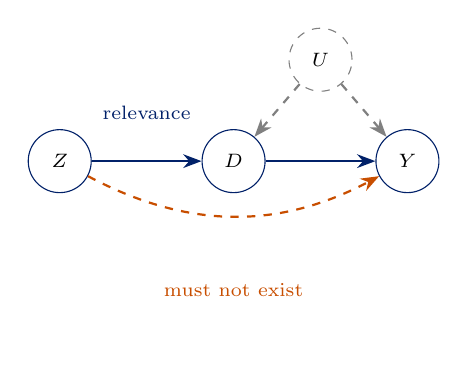
\begin{tikzpicture}[scale=0.92,>=Stealth,
  every node/.style={circle,draw=dukeblue,fill=white,inner sep=1pt,minimum size=8mm,font=\scriptsize}]
  \node (z) at (0,0) {$Z$};  \node (d) at (2.4,0) {$D$};  \node (y) at (4.8,0) {$Y$};
  \node[draw=gray,dashed] (u) at (3.6,1.4) {$U$};
  \draw[->,dukeblue,thick] (z)--(d) node[draw=none,fill=none,midway,above,font=\scriptsize]{relevance};
  \draw[->,dukeblue,thick] (d)--(y);
  \draw[->,gray,dashed,thick] (u)--(d); \draw[->,gray,dashed,thick] (u)--(y);
  \draw[->,accent,dashed,thick] (z) to[bend right=28] node[draw=none,fill=none,midway,below,font=\scriptsize,text=accent]{must not exist} (y);
\end{tikzpicture}
\end{center}
\vskip-8pt
\begin{block}{Three conditions, stated carefully}
\begin{enumerate}\itemsep1pt
  \item \textbf{Relevance}: $\Cov(Z_i, D_i) \neq 0$. \alert{Testable.}
  \item \textbf{Independence}: $Z_i$ is as good as randomly assigned --- no
        arrow into $Z$ from anything that also causes $Y$.
  \item \textbf{Exclusion}: $Z$ affects $Y$ \emph{only} through $D$. \alert{Not
        testable.}
\end{enumerate}
\end{block}
\vskip2pt
Conditions 2 and 3 are distinct and are often conflated. A randomized lottery
satisfies 2 by construction and can still violate 3.
\end{frame}

\begin{frame}{The Wald Estimator}
Take covariances of $Y_i = \alpha + \beta D_i + \epsilon_i$ with $Z_i$:
\begin{align*}
  \Cov(Z_i, Y_i) = \beta\,\Cov(Z_i,D_i) + \underbrace{\Cov(Z_i,\epsilon_i)}_{=\,0}
  \quad\Longrightarrow\quad
  \boxed{\;\beta_{IV} = \frac{\Cov(Z_i,Y_i)}{\Cov(Z_i,D_i)}\;}
\end{align*}
\pause
With a \emph{binary} instrument this is a ratio of two differences in means:
\begin{align*}
  \beta_{IV}
  = \frac{\E[Y_i\mid Z_i=1] - \E[Y_i\mid Z_i = 0]}
         {\E[D_i\mid Z_i=1] - \E[D_i\mid Z_i = 0]}
  = \frac{\text{reduced form}}{\text{first stage}} .
\end{align*}
\vskip2pt
Read it as: \emph{the effect of the instrument on the outcome, scaled up by how
much the instrument moved the treatment.}
\end{frame}

\begin{frame}{Intuition for the Ratio}
Divide numerator and denominator by $\Var(Z_i)$:
\begin{align*}
  \beta_{IV}
  = \frac{\Cov(Z_i,Y_i)/\Var(Z_i)}{\Cov(Z_i,D_i)/\Var(Z_i)}
  = \frac{\text{coefficient from regressing } Y \text{ on } Z}
         {\text{coefficient from regressing } D \text{ on } Z} .
\end{align*}
\begin{center}
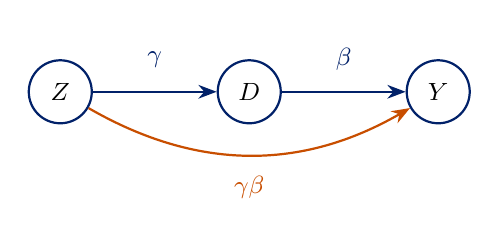
\begin{tikzpicture}[scale=1.0,>=Stealth,thick,
  every node/.style={circle,draw=dukeblue,fill=white,inner sep=1pt,minimum size=8mm,font=\small}]
  \node (Z) at (0,0) {$Z$}; \node (D) at (2.4,0) {$D$}; \node (Y) at (4.8,0) {$Y$};
  \draw[->,dukeblue] (Z)--(D) node[draw=none,fill=none,midway,above]{\small$\gamma$};
  \draw[->,dukeblue] (D)--(Y) node[draw=none,fill=none,midway,above]{\small$\beta$};
  \draw[->,accent] (Z) to[bend right=30] node[draw=none,fill=none,midway,below,text=accent]{\small$\gamma\beta$} (Y);
\end{tikzpicture}
\end{center}
\vskip-6pt
\begin{itemize}\itemsep2pt
  \item The instrument's total effect on $Y$ travels along one path and equals
        $\gamma\beta$. The first stage recovers $\gamma$. Dividing isolates
        $\beta$.
  \item \alert{If $\gamma$ is small, we are dividing by something close to zero.}
        Hold that thought --- it is the whole of the weak-instrument problem.
\end{itemize}
\end{frame}

%%%%%%%%%%%%%%%%%%%%%%%%%%%%%%%%%%%%%%%%%%%%%%%%%%%%%%%%%%%%%%%%%%%%%%%%%%%%%%%
\section[Applications]{Two Canonical Applications}
%%%%%%%%%%%%%%%%%%%%%%%%%%%%%%%%%%%%%%%%%%%%%%%%%%%%%%%%%%%%%%%%%%%%%%%%%%%%%%%
\begin{frame}\sectionpage\end{frame}

\begin{frame}{Settler Mortality and Institutions}
\srct{Acemoglu, Johnson, and Robinson (2001)} estimate the effect of institutional
quality ($D$, protection from expropriation risk) on GDP per capita ($Y$).
\vskip3pt
\begin{itemize}\itemsep3pt
  \item Institutions are obviously endogenous to economic performance: rich
        countries can afford good institutions, and both may be driven by
        culture, geography, or history.
  \item \textbf{The instrument}: mortality rates faced by European settlers in the
        colonial period.
  \item \textbf{The mechanism argument}: where settlers could survive, they
        settled and built inclusive institutions --- property rights, rule of law.
        Where mortality was high, colonization was extractive. Those institutional
        forms persisted long after the disease environment ceased to matter.
  \item \textbf{Relevance}: strongly supported by the first stage.
\end{itemize}
\end{frame}

\begin{frame}{Where the AJR Argument Is Attacked}
Exclusion requires that historical settler mortality affects income \emph{today}
only through institutions.
\vskip3pt
\begin{itemize}\itemsep3pt
  \item \alert{The leading threat is geography.} The disease environment that
        killed settlers also shapes agricultural productivity, the modern disease
        burden, and human capital --- all of which affect income directly.
  \item AJR's response is an \emph{assumption}: that the confounding role of
        geography is adequately captured by a linear term in distance from the
        equator plus continent dummies.
  \item That is a functional-form assumption doing identification work, and it
        is rarely defended. We come back to it briefly in Week 13.
  \item Subsequent critiques questioned the mortality data itself. \alert{Note
        the pattern}: exclusion cannot be tested, so the debate becomes a debate
        about history, measurement, and functional form. That is healthy, and it
        is what IV papers should invite.
\end{itemize}
\end{frame}

\begin{frame}{Quarter of Birth and Schooling}
\srct{Angrist and Krueger (1991)} estimate the return to schooling using
\textbf{quarter of birth} as an instrument.
\vskip3pt
\begin{itemize}\itemsep3pt
  \item \textbf{The mechanism}: children start school in the year they turn six,
        but may leave at a fixed \emph{age} (16 or 17). Those born early in the
        calendar year reach the leaving age having completed less schooling.
  \item \textbf{Relevance}: the first stage is real but small --- a fraction of a
        year of schooling.
  \item \textbf{Exclusion}: birth quarter should not affect earnings except
        through schooling. Contested, because season of birth correlates with
        maternal characteristics, health at birth, and relative age in class.
  \item \textbf{The compliers} are people who would have dropped out at the
        minimum age. The LATE is therefore a return to schooling \emph{at the
        bottom of the schooling distribution} --- a different quantity from the
        average return, and arguably the policy-relevant one for compulsory
        attendance laws.
\end{itemize}
\end{frame}

\begin{frame}[shrink=10]{The Cautionary Half of Angrist--Krueger}
The paper is also the standard illustration of what goes wrong with many weak
instruments.
\vskip3pt
\begin{itemize}\itemsep3pt
  \item To gain precision, the authors interacted quarter of birth with state and
        year of birth, producing up to 180 instruments.
  \item \srct{Bound, Jaeger, and Baker (1995)} showed that with that many weak
        instruments, 2SLS is biased \emph{toward OLS}, and demonstrated it
        devastatingly: replacing quarter of birth with \emph{randomly generated}
        instruments produced similar estimates and standard errors.
  \item The mechanism is overfitting the first stage. $\hat D$ starts to
        reproduce the endogenous variation we were trying to discard.
  \item \alert{More instruments is not more information.} Report the just-identified
        estimate alongside any overidentified one.
\end{itemize}
\vskip2pt
Sociological instruments worth knowing: sibling sex composition for fertility,
distance to college for schooling, lottery admission for school quality, and the
draft lottery for military service.
\end{frame}

%%%%%%%%%%%%%%%%%%%%%%%%%%%%%%%%%%%%%%%%%%%%%%%%%%%%%%%%%%%%%%%%%%%%%%%%%%%%%%%
\section[2SLS]{Two-Stage Least Squares}
%%%%%%%%%%%%%%%%%%%%%%%%%%%%%%%%%%%%%%%%%%%%%%%%%%%%%%%%%%%%%%%%%%%%%%%%%%%%%%%
\begin{frame}\sectionpage\end{frame}

\begin{frame}{The Two Stages}
With covariates and possibly several instruments:
\begin{align*}
  \text{Stage 1:}\quad D_i &= \pi_0 + \pi_1 Z_i + \pi_2' W_i + v_i
  \quad\Longrightarrow\quad \hat D_i \\[3pt]
  \text{Stage 2:}\quad Y_i &= \alpha + \beta \hat D_i + \gamma' W_i + u_i
\end{align*}
\vskip3pt
\begin{itemize}\itemsep3pt
  \item $\hat D_i$ is the part of $D_i$ \emph{explained by the instrument}, which
        by assumption is uncorrelated with $\epsilon_i$. We regress on the clean
        part and discard the rest.
  \item \alert{The exogenous covariates $W_i$ must appear in \emph{both} stages.}
        Omitting them from the first stage is a common and serious error.
  \item \textbf{Order condition}: at least as many excluded instruments as
        endogenous regressors. \emph{Exactly identified} means equality;
        \emph{overidentified} means more.
  \item \alert{Never run the two stages by hand.} The second-stage standard errors
        would treat $\hat D$ as data rather than as an estimate. Use
        \texttt{ivreg()} or \texttt{feols(y \textasciitilde\ w | d \textasciitilde\ z)}.
\end{itemize}
\end{frame}

\begin{frame}[shrink=10]{IV in Matrix Form\adv}
Start from the moment condition $\E[\bm Z' u] = \zero$ with $Y = D\beta_0 + u$.
The sample analogue $\bm Z'(\bm Y - \bm D\hat\beta) = \zero$ has no solution
when there are more instruments than regressors, so instead \emph{minimize} the
sample moments in a weighted norm:
\begin{align*}
  \hat\beta = \argmin_{b}\ \big(\bm Z'(\bm Y-\bm Db)\big)'
  (\bm Z'\bm Z)^{-1}\big(\bm Z'(\bm Y-\bm Db)\big) .
\end{align*}
The first-order condition gives
\begin{align*}
  \hat\beta = \Big(\bm D'\bm Z(\bm Z'\bm Z)^{-1}\bm Z'\bm D\Big)^{-1}
              \bm D'\bm Z(\bm Z'\bm Z)^{-1}\bm Z'\bm Y .
\end{align*}
\pause
Define the projection matrix $\bm P_Z = \bm Z(\bm Z'\bm Z)^{-1}\bm Z'$ --- the
same object as Week 1, now projecting onto the instrument space:
\begin{align*}
  \boxed{\;\hat\beta_{2SLS} = \big(\bm D'\bm P_Z \bm D\big)^{-1}\bm D'\bm P_Z\bm Y\;}
\end{align*}
Since $\bm P_Z\bm D$ \emph{is} the first-stage fitted value and $\bm P_Z$ is
idempotent, this is literally ``regress $\bm Y$ on $\hat{\bm D}$.'' And when
$\bm Z = \bm D$, $\bm P_Z\bm D = \bm D$ and 2SLS collapses to OLS: \alert{OLS is
the special case in which you claim everything is exogenous}.
\end{frame}

\begin{frame}{The IV Sandwich\adv}
Substitute $\bm Y = \bm D\beta_0 + \bm u$:
\begin{align*}
  \hat\beta - \beta_0 = \big(\bm D'\bm P_Z\bm D\big)^{-1}\bm D'\bm P_Z \bm u .
\end{align*}
Multiply by $\sqrt n$. Under regularity conditions and a \emph{strong}
instrument,
\begin{align*}
  \tfrac1n \bm D'\bm P_Z\bm D \pto \bm A \succ 0,
  \qquad
  \tfrac{1}{\sqrt n}\bm D'\bm P_Z\bm u \dto \mathcal N(\zero, \bm S) ,
\end{align*}
so by Slutsky $\sqrt n(\hat\beta-\beta_0)\dto \mathcal N(\zero, \bm A^{-1}\bm S\bm A^{-1})$.
\vskip3pt
The robust variance estimator is the familiar sandwich:
\begin{align*}
  \widehat{\Var}(\hat\beta)
  = (\bm D'\bm P_Z\bm D)^{-1}\,\bm D'\bm P_Z\,
    \widehat{\Var}(\bm u)\,\bm P_Z\bm D\,(\bm D'\bm P_Z\bm D)^{-1} ,
\end{align*}
plugging in $\widehat{\Var}(\bm u) = \mathrm{diag}(\hat u_i^2)$ --- and clustering
exactly as in Week 2. \alert{Note the residuals $\hat u_i$ must be computed with
the actual $D_i$, not $\hat D_i$}; this is the other reason not to run the stages
by hand.
\end{frame}

%%%%%%%%%%%%%%%%%%%%%%%%%%%%%%%%%%%%%%%%%%%%%%%%%%%%%%%%%%%%%%%%%%%%%%%%%%%%%%%
\section[LATE]{What Does IV Estimate?}
%%%%%%%%%%%%%%%%%%%%%%%%%%%%%%%%%%%%%%%%%%%%%%%%%%%%%%%%%%%%%%%%%%%%%%%%%%%%%%%
\begin{frame}\sectionpage\end{frame}

\begin{frame}[shrink=10]{Four Types of People}
With a binary instrument and binary treatment, write $D_i(z)$ for the treatment
unit $i$ would take if assigned $Z_i = z$. Every unit is one of four types:
\begin{center}\small
\renewcommand{\arraystretch}{1.25}
\begin{tabular}{lccl}
\toprule
Type & $D_i(0)$ & $D_i(1)$ & \\
\midrule
\textbf{Compliers} & 0 & 1 & do what the instrument says \\
Always-takers & 1 & 1 & treated regardless \\
Never-takers & 0 & 0 & untreated regardless \\
\alert{Defiers} & 1 & 0 & do the opposite \\
\bottomrule
\end{tabular}
\end{center}
\vskip4pt
\begin{itemize}\itemsep2pt
  \item We never observe anyone's type: we see $D_i(1)$ or $D_i(0)$, never both.
        Type is a latent variable, and this is the same fundamental problem as
        Week 5, one level up.
  \item Only \textbf{compliers} have their treatment moved by the instrument.
  \item \alert{Monotonicity} assumes there are no defiers: the instrument pushes
        everyone in the same direction, or not at all.
\end{itemize}
\end{frame}

\begin{frame}{Deriving the LATE: the Numerator}
Write the reduced form using the switching equation
$Y_i = Y_i\big(D_i(Z_i)\big)$ and split by type. Because $Z$ is independent of
potential outcomes and types,
\begin{align*}
  &\E[Y_i\mid Z_i=1] - \E[Y_i\mid Z_i=0] \\
  &\quad= \Pr(\text{AT})\underbrace{\big(\E[Y_i(1)\mid \text{AT}] - \E[Y_i(1)\mid \text{AT}]\big)}_{=\,0} \\
  &\quad\ + \Pr(\text{NT})\underbrace{\big(\E[Y_i(0)\mid \text{NT}] - \E[Y_i(0)\mid \text{NT}]\big)}_{=\,0} \\
  &\quad\ + \Pr(\text{C})\ \big(\E[Y_i(1)\mid \text{C}] - \E[Y_i(0)\mid \text{C}]\big) \\
  &\quad\ - \Pr(\text{D})\ \big(\E[Y_i(1)\mid \text{D}] - \E[Y_i(0)\mid \text{D}]\big) .
\end{align*}
\vskip2pt
Always- and never-takers take the \emph{same} treatment under both values of
$Z$, so \alert{by exclusion} their outcomes are unchanged and they contribute
zero. \alert{Monotonicity} kills the last line by assuming $\Pr(\text{D})=0$ ---
note that defiers would enter with the \emph{wrong sign}.
\end{frame}

\begin{frame}{Deriving the LATE: the Denominator}
The first stage recovers the complier share:
\begin{align*}
  \E[D_i\mid Z_i=1] - \E[D_i\mid Z_i=0]
  &= \Pr(\text{C}) + \Pr(\text{AT}) - \big(\Pr(\text{AT})\big) \\
  &= \Pr(\text{C}) .
\end{align*}
\vskip3pt
Dividing:
\begin{block}{The LATE theorem \srcp{Imbens and Angrist 1994}}
\begin{align*}
  \frac{\E[Y\mid Z=1] - \E[Y\mid Z=0]}{\E[D\mid Z=1]-\E[D\mid Z=0]}
  = \E\big[\,Y_i(1) - Y_i(0)\ \big|\ \text{$i$ is a complier}\,\big] .
\end{align*}
\end{block}
\vskip3pt
\alert{IV does not estimate the ATE.} It estimates the average effect for the
subpopulation whose treatment status the instrument actually changed --- a group
you cannot identify by name, defined by the instrument you happened to choose.
\end{frame}

\begin{frame}{Living With the LATE}
\begin{itemize}\itemsep3pt
  \item If effects are homogeneous, LATE $=$ ATE and none of this matters. That is
        rarely a defensible assumption in sociology.
  \item Different instruments for the same treatment estimate \emph{different}
        LATEs. When two IV papers disagree, that is not necessarily a
        contradiction --- it may be two correct answers to two different questions.
  \item \textbf{You can describe the compliers even though you cannot name them}:
        their share is the first stage, and their covariate means are recoverable
        by reweighting (Abadie's $\kappa$).
  \item \textbf{Compliers are often unusual}: for quarter-of-birth they are
        marginal dropouts; for judge-leniency designs they are defendants near the
        decision margin. Whether that group is the policy-relevant one is a
        substantive question you must answer, not a technicality.
\end{itemize}
\vskip2pt
\alert{Always characterize your compliers.} It is the difference between an
interpretable LATE and a number.
\end{frame}

%%%%%%%%%%%%%%%%%%%%%%%%%%%%%%%%%%%%%%%%%%%%%%%%%%%%%%%%%%%%%%%%%%%%%%%%%%%%%%%
\section[Weak IV]{Weak Instruments and Inference}
%%%%%%%%%%%%%%%%%%%%%%%%%%%%%%%%%%%%%%%%%%%%%%%%%%%%%%%%%%%%%%%%%%%%%%%%%%%%%%%
\begin{frame}\sectionpage\end{frame}

\begin{frame}{Weak Instruments Are Worse Than No Instrument}
Recall $\hat\beta_{IV} = \widehat\Cov(Z,Y)/\widehat\Cov(Z,D)$. If the denominator
is near zero, small violations of exclusion get \emph{divided by} a small number:
\begin{align*}
  \plim \hat\beta_{IV} = \beta + \frac{\Cov(Z,\epsilon)}{\Cov(Z,D)} .
\end{align*}
\vskip3pt
\begin{itemize}\itemsep3pt
  \item An instrument that is one-tenth as endogenous as $D$ but one-hundredth as
        strongly correlated with it produces \alert{more} bias than plain OLS.
  \item In matrix terms\adv, the variance depends on
        $(\bm D'\bm P_Z\bm D)^{-1}$. If the instruments explain little of $\bm D$
        that matrix is small and its inverse is large.
  \item Worse, under weak identification $\hat\beta_{2SLS}$ has \alert{no Gaussian
        limit}: the limiting distribution is non-normal and heavy-tailed, so the
        conventional $t$-test fails no matter how large $n$ is.
  \item The problem \emph{worsens} with more instruments, because many weak
        instruments overfit the first stage --- the Bound--Jaeger--Baker point.
\end{itemize}
\end{frame}

\begin{frame}{Diagnosing Instrument Strength}
\begin{itemize}\itemsep3pt
  \item \textbf{First-stage $F$} on the excluded instruments. The traditional rule
        of thumb is $F > 10$ \srcp{Staiger and Stock 1997; Stock and Yogo 2005},
        derived so that 2SLS bias is under 10\% of OLS bias.
  \item \alert{That rule is about bias, not about test size, and it is now known
        to be far too lax for inference.}
        \srct{Lee, McCrary, Moreira, and Porter (2022)} show that a conventional
        $5\%$ $t$-test has correct size only when the first-stage $F$ exceeds
        roughly \textbf{104}. Their \texttt{tF} procedure replaces the $1.96$
        critical value with a larger one read off $F$: at $F = 10$ the adjusted
        critical value is about \textbf{3.43}, so the honest interval is roughly
        \textbf{1.75} times wider than the printed one.
  \item Use a \emph{robust} first-stage $F$ if you use robust or clustered
        standard errors in the second stage.
  \item With several endogenous regressors, use the \emph{Kleibergen--Paap} rank
        statistic; a strong $F$ on each instrument separately is not enough.
\end{itemize}
\end{frame}

\begin{frame}{Anderson--Rubin: Inference That Never Divides}
The problem is the division by a noisy first stage. \srct{Anderson and Rubin
(1949)} avoid it by testing the moment condition directly.
\vskip3pt
To test $H_0: \beta = \beta_0$, note that under the null
$\E\big[(Y_i - \beta_0 D_i)Z_i\big] = 0$. Form the statistic
\begin{align*}
  C(\beta_0) = \frac{\Big|\En\big[(Y_i - \beta_0 D_i)\,Z_i\big]\Big|^2}
                    {\widehat{\Var}_n\big[(Y_i-\beta_0D_i)Z_i\big]/n}
  \ \dto\ \chi^2_1 \quad\text{under } H_0 ,
\end{align*}
(with variables residualized on any exogenous controls first). Reject at level
$a$ if $C(\beta_0) > c_{1-a}$, the $(1-a)$ quantile of $\chi^2_1$.
\vskip3pt
\begin{itemize}\itemsep2pt
  \item Operationally: regress $Y_i - \beta_0 D_i$ on the instruments and test
        whether their coefficients are jointly zero.
  \item \alert{The first stage never appears in the denominator}, so the test is
        valid whatever the instrument's strength.
\end{itemize}
\end{frame}

\begin{frame}[shrink=10]{Inverting the Test}
A confidence region is the set of null values the data cannot reject:
\begin{align*}
  CR(\beta) = \big\{\beta_0 \in \Theta : C(\beta_0) \leq c_{1-a}\big\} .
\end{align*}
In practice: grid over $\beta_0$, compute $C(\beta_0)$, keep the values that
survive.
\vskip3pt
\begin{itemize}\itemsep3pt
  \item The region can be an interval, a \emph{union} of disjoint intervals, the
        whole real line, or \emph{empty}. None of these is a bug.
  \item An \textbf{unbounded} region is the honest statement that the data cannot
        pin $\beta$ down --- which is precisely what a conventional interval hides
        when the instrument is weak.
  \item An \textbf{empty} region can arise only when the model is
        \emph{overidentified} --- with one instrument and one endogenous regressor
        the 2SLS value always satisfies the moment exactly. When it does happen it
        is evidence against the overidentifying restrictions.
  \item \texttt{ivmodel}, \texttt{ivDiag}, or a hand-coded grid --- it is ten
        lines of code, and we write them in lab.
\end{itemize}
\end{frame}

\begin{frame}{Overidentification Tests: Read Them Carefully}
With more instruments than endogenous regressors, the Sargan--Hansen $J$ test
asks whether the instruments agree with one another.
\vskip3pt
\begin{itemize}\itemsep3pt
  \item \textbf{Rejection} says at least one instrument is invalid --- \emph{or}
        that effects are heterogeneous, so the instruments estimate different
        LATEs and are supposed to disagree. It does not say which.
  \item \textbf{Non-rejection is nearly worthless.} It is consistent with all the
        instruments being invalid \emph{in the same direction}, and the test has
        little power.
  \item The $J$ test cannot validate exclusion. Nothing can. The defence is
        substantive: tell a story about why $Z$ could not affect $Y$ except
        through $D$, and look for \emph{placebo outcomes} it should not move and
        \emph{placebo samples} in which the first stage should be absent.
\end{itemize}
\end{frame}

%%%%%%%%%%%%%%%%%%%%%%%%%%%%%%%%%%%%%%%%%%%%%%%%%%%%%%%%%%%%%%%%%%%%%%%%%%%%%%%
\section[Practice]{Practice}
%%%%%%%%%%%%%%%%%%%%%%%%%%%%%%%%%%%%%%%%%%%%%%%%%%%%%%%%%%%%%%%%%%%%%%%%%%%%%%%
\begin{frame}\sectionpage\end{frame}

\begin{frame}[shrink=10]{A Reader's Checklist}
Adapted from \srct{Sovey and Green (2011)}. Any IV paper should report:
\begin{enumerate}\itemsep2pt
  \item The instrument, and an explicit argument for exclusion --- not just a
        citation to a prior paper that used it.
  \item The \textbf{first stage}, its coefficient, and its robust $F$.
  \item The \textbf{reduced form} ($Y$ on $Z$), with its estimate and interval.
        It needs no instrument-strength assumption, so it is the most robust piece
        of evidence in the design --- and if it is indistinguishable from zero the
        IV estimate rests on very little.
  \item The \textbf{OLS} estimate alongside, so the reader can see the direction
        and size of the correction --- and whether it goes the way theory predicts.
  \item Who the \textbf{compliers} are, and their share.
  \item Weak-instrument-robust inference if $F$ is not comfortably large.
  \item The just-identified estimate if the paper is overidentified.
  \item Placebo checks: outcomes and subgroups $Z$ should not affect.
\end{enumerate}
\vskip2pt
\alert{If a paper reports only the 2SLS coefficient, that is a red flag.}
\end{frame}

\begin{frame}[shrink=10]{When IV Is the Wrong Tool}
\begin{itemize}\itemsep3pt
  \item \textbf{No credible instrument exists.} This is the normal state of
        affairs. An implausible instrument is worse than an honest
        selection-on-observables analysis with sensitivity bounds.
  \item \textbf{The LATE is not the quantity of interest.} If your policy question
        concerns always-takers, the compliers' effect does not answer it.
  \item \textbf{Interpretation drifts.} Papers routinely estimate a LATE and then
        discuss it as if it were an ATE.
  \item \textbf{Monotonicity is doing hidden work.} In judge-leniency and
        examiner designs, it must hold for \emph{every} judge simultaneously ---
        a much stronger claim than it first appears.
\end{itemize}
\vskip3pt
\begin{block}{The design-based cousins}
When the instrument is a discontinuity in an assignment rule, you have
\textbf{RDD} (Week 9) --- and indeed fuzzy RD \emph{is} local IV. When it is a
policy change over time, you have \textbf{DID} (Week 10).
\end{block}
\end{frame}

\begin{frame}{Looking Ahead}
\begin{itemize}\itemsep4pt
  \item IV replaces ``I measured all confounders'' with ``I found variation that
        is as good as random.'' Both are assumptions; the second is easier to
        argue about substantively, and easier for readers to attack --- which is
        a virtue.
  \item The price is the estimand: LATE, for compliers you cannot name, defined
        by the instrument you chose.
  \item Notice how much identification work was done by \emph{functional form} in
        AJR --- ``linear in distance from the equator, plus continent dummies.''
        Week 13 asks briefly what can be done when you are unwilling to assume
        that.
\end{itemize}
\vskip3pt
\begin{block}{Midterm}
\textbf{Thursday, October 15}, in class, covering Weeks 1--7. Open book and open
note, timed, no coding. Tuesday October 13 is Fall break.
\end{block}
\end{frame}

\begin{frame}[allowframebreaks]{References}
\footnotesize
\begin{itemize}\itemsep3pt
\item Acemoglu, Daron, Simon Johnson, and James A. Robinson. 2001. ``The Colonial
Origins of Comparative Development.'' \textit{American Economic Review} 91(5):
1369--1401.
\item Angrist, Joshua D. and Alan B. Krueger. 1991. ``Does Compulsory School
Attendance Affect Schooling and Earnings?'' \textit{Quarterly Journal of
Economics} 106(4): 979--1014.
\item Angrist, Joshua D., Guido W. Imbens, and Donald B. Rubin. 1996.
``Identification of Causal Effects Using Instrumental Variables.''
\textit{Journal of the American Statistical Association} 91(434): 444--455.
\item Anderson, T.W. and Herman Rubin. 1949. ``Estimation of the Parameters of a
Single Equation in a Complete System of Stochastic Equations.''
\textit{Annals of Mathematical Statistics} 20(1): 46--63.
\item Angrist, Joshua D. and J\"orn-Steffen Pischke. 2009.
\textit{Mostly Harmless Econometrics}. Princeton University Press. [Ch.\ 4]
\item Bound, John, David A. Jaeger, and Regina M. Baker. 1995. ``Problems with
Instrumental Variables Estimation When the Correlation Between the Instruments
and the Endogenous Explanatory Variable Is Weak.'' \textit{Journal of the
American Statistical Association} 90(430): 443--450.
\item Imbens, Guido W. and Joshua D. Angrist. 1994. ``Identification and
Estimation of Local Average Treatment Effects.'' \textit{Econometrica} 62(2):
467--475.
\item Lee, David S., Justin McCrary, Marcelo J. Moreira, and Jack Porter. 2022.
``Valid $t$-Ratio Inference for IV.'' \textit{American Economic Review} 112(10):
3260--3290.
\item Morgan, Stephen L. and Christopher Winship. 2015.
\textit{Counterfactuals and Causal Inference}, 2nd ed. Cambridge University
Press. [Ch.\ 9]
\item Sovey, Allison J. and Donald P. Green. 2011. ``Instrumental Variables
Estimation in Political Science: A Reader's Guide.'' \textit{American Journal of
Political Science} 55(1): 188--200.
\item Stock, James H. and Motohiro Yogo. 2005. ``Testing for Weak Instruments in
Linear IV Regression.'' In \textit{Identification and Inference for Econometric
Models}, ed. Andrews and Stock. Cambridge University Press, 80--108.
\item Staiger, Douglas and James H. Stock. 1997. ``Instrumental Variables
Regression with Weak Instruments.'' \textit{Econometrica} 65(3): 557--586.
\end{itemize}
\end{frame}

\end{document}
